\documentclass[10pt, aspectratio=169]{beamer}

\usetheme[progressbar=frametitle]{metropolis}
\usefonttheme{serif}
\setbeamertemplate{frame numbering}[none]
\useoutertheme{metropolis}
\useinnertheme{metropolis}
%\usecolortheme{beaver}
\setbeamercolor{background canvas}{bg=white}

\usepackage[italian]{babel}
\usepackage[utf8]{inputenc}

\usepackage{multicol}
\usepackage{parskip}[5pt]

\title[Titolo in basso a destra]{Lezioni di Matematica: Derivate}
\subtitle{sottotitolo lezione}
\date{\today}
\author{prof. Diego Fantinelli}
\institute{Matematica per il Liceo}

\begin{document}
\metroset{block=fill}

\begin{frame}
	\titlepage
\end{frame}

\begin{frame}
\frametitle{contenuti}
	\tableofcontents
\end{frame}

\section{Derivate: introduzione e definizioni}

\begin{frame}[t]{Derivate - introduzione} \vspace{10pt}
\begin{alertblock}{Esercizio 1. (a)}
\textcolor{magenta}{Tre fari si accendono ad intervalli regolari. Il primo si accende ogni 8 s, il secondo faro ogni 12 s, il terzo ogni 15 s. Se ad un certo istante si accendono contemporaneamente, dopo quanti secondi torneranno ad accendersi insieme?}\\  \vspace{8pt}
I secondi che dovranno passare per far s� che i tre fari si accendano contemporaneamente
dovranno essere un multiplo di 8, 12 e 15, il minimo comune multiplo.
Effettuata la scomposizione in fattori primi, risulta che:
\begin{align*}
	8 & = 2^3\\
	12 & = 2^2 \cdot 3\\
	15 & = 3 \cdot 5
\end{align*}
per cui il \(m.c.m. = 2^3 \cdot 3 \cdot 5 = 120 \)\\
I tre fari torneranno ad accendersi contemporaneamente dopo 120 secondi.
\end{alertblock}
\end{frame}

\begin{frame}
\begin{definition} \vspace{2pt}
A prime number is a number that...
\end{definition}

\begin{example} \vspace{2pt}
Lorem ipsum dolor sit amet, consectetur adipisicing elit, 
sed do eiusmod tempor incididunt ut labore et
dolore magna aliqua.
\end{example}
\end{frame}


\begin{frame}[t]{Derivate - Rappresentazione grafica} \vspace{5pt}
Liste numerate e puntate su 2 colonne:\\ \textcolor{magenta}{$a^2+b^2=c^2$}, e capiremo come cambiare la prospettiva con cui si osserva una formula matematica\\
\begin{multicols}{2}
	
\begin{enumerate}
	\item primo elemento
	\begin{enumerate}
		\item uno
		\item due
	\end{enumerate}
	\item secondo elemento
	\item terzo elemento
\end{enumerate}

\begin{itemize}
	\item primo elemento
		\begin{itemize}
			\item secondo elemento
			\item terzo di tre
		\end{itemize}
	\item terzo elemento
\end{itemize}
\end{multicols}
\end{frame}

%\begin{frame}[t]{Definizioni} \vspace{10pt}
%\begin{block}{Funzione}
%\vspace{0.5em}
%In questa lezione vedremo come analizzare la scrittura: $a^2+b^2=c^2$, e capiremo come cambiare la prospettiva con cui si osserva una formula matematica
%\vspace{0.5em}	
%
%\end{block}
%\end{frame}

\section{Esercitazioni}
\begin{frame}[t]{Esercizi sulle derivate} \vspace{10pt}
	\begin{theorem}\vspace{2pt}
         Let $r, s$ be integers such that gcd$(r, s)=1$. 
         $\displaystyle \int_{0}^{\infty}x^2 - 6 x + 49 \cdot dx$ \\
         Given integers $a,b$, there exists unique 
        $x <rs$ such that 
        \begin{enumerate}
        		\item primo elemento
		\begin{itemize}
			\item secondo elemento
			\item terzo di tre
		\end{itemize}
	\item terzo elemento
\end{enumerate}
	\end{theorem}
\vspace{5pt}
        
\begin{block}{semplice blocco di testo} \vspace{2pt}
Lorem ipsum dolor sit amet, consectetur adipisicing elit, 
sed do eiusmod tempor incididunt ut labore et 
dolore magna aliqua.
\end{block}
\end{frame}

\begin{frame}[t]{Esercizi sulle derivate} \vspace{10pt}
\begin{multicols}{2}
Hello, here is some text without a meaning.  If you read this text, you will get no information.\\ $\displaystyle \int_{0}^{\infty}x^2 - 6 x + 49 \cdot dx$, you will get no information
If you read this text, you will get no information. \\ 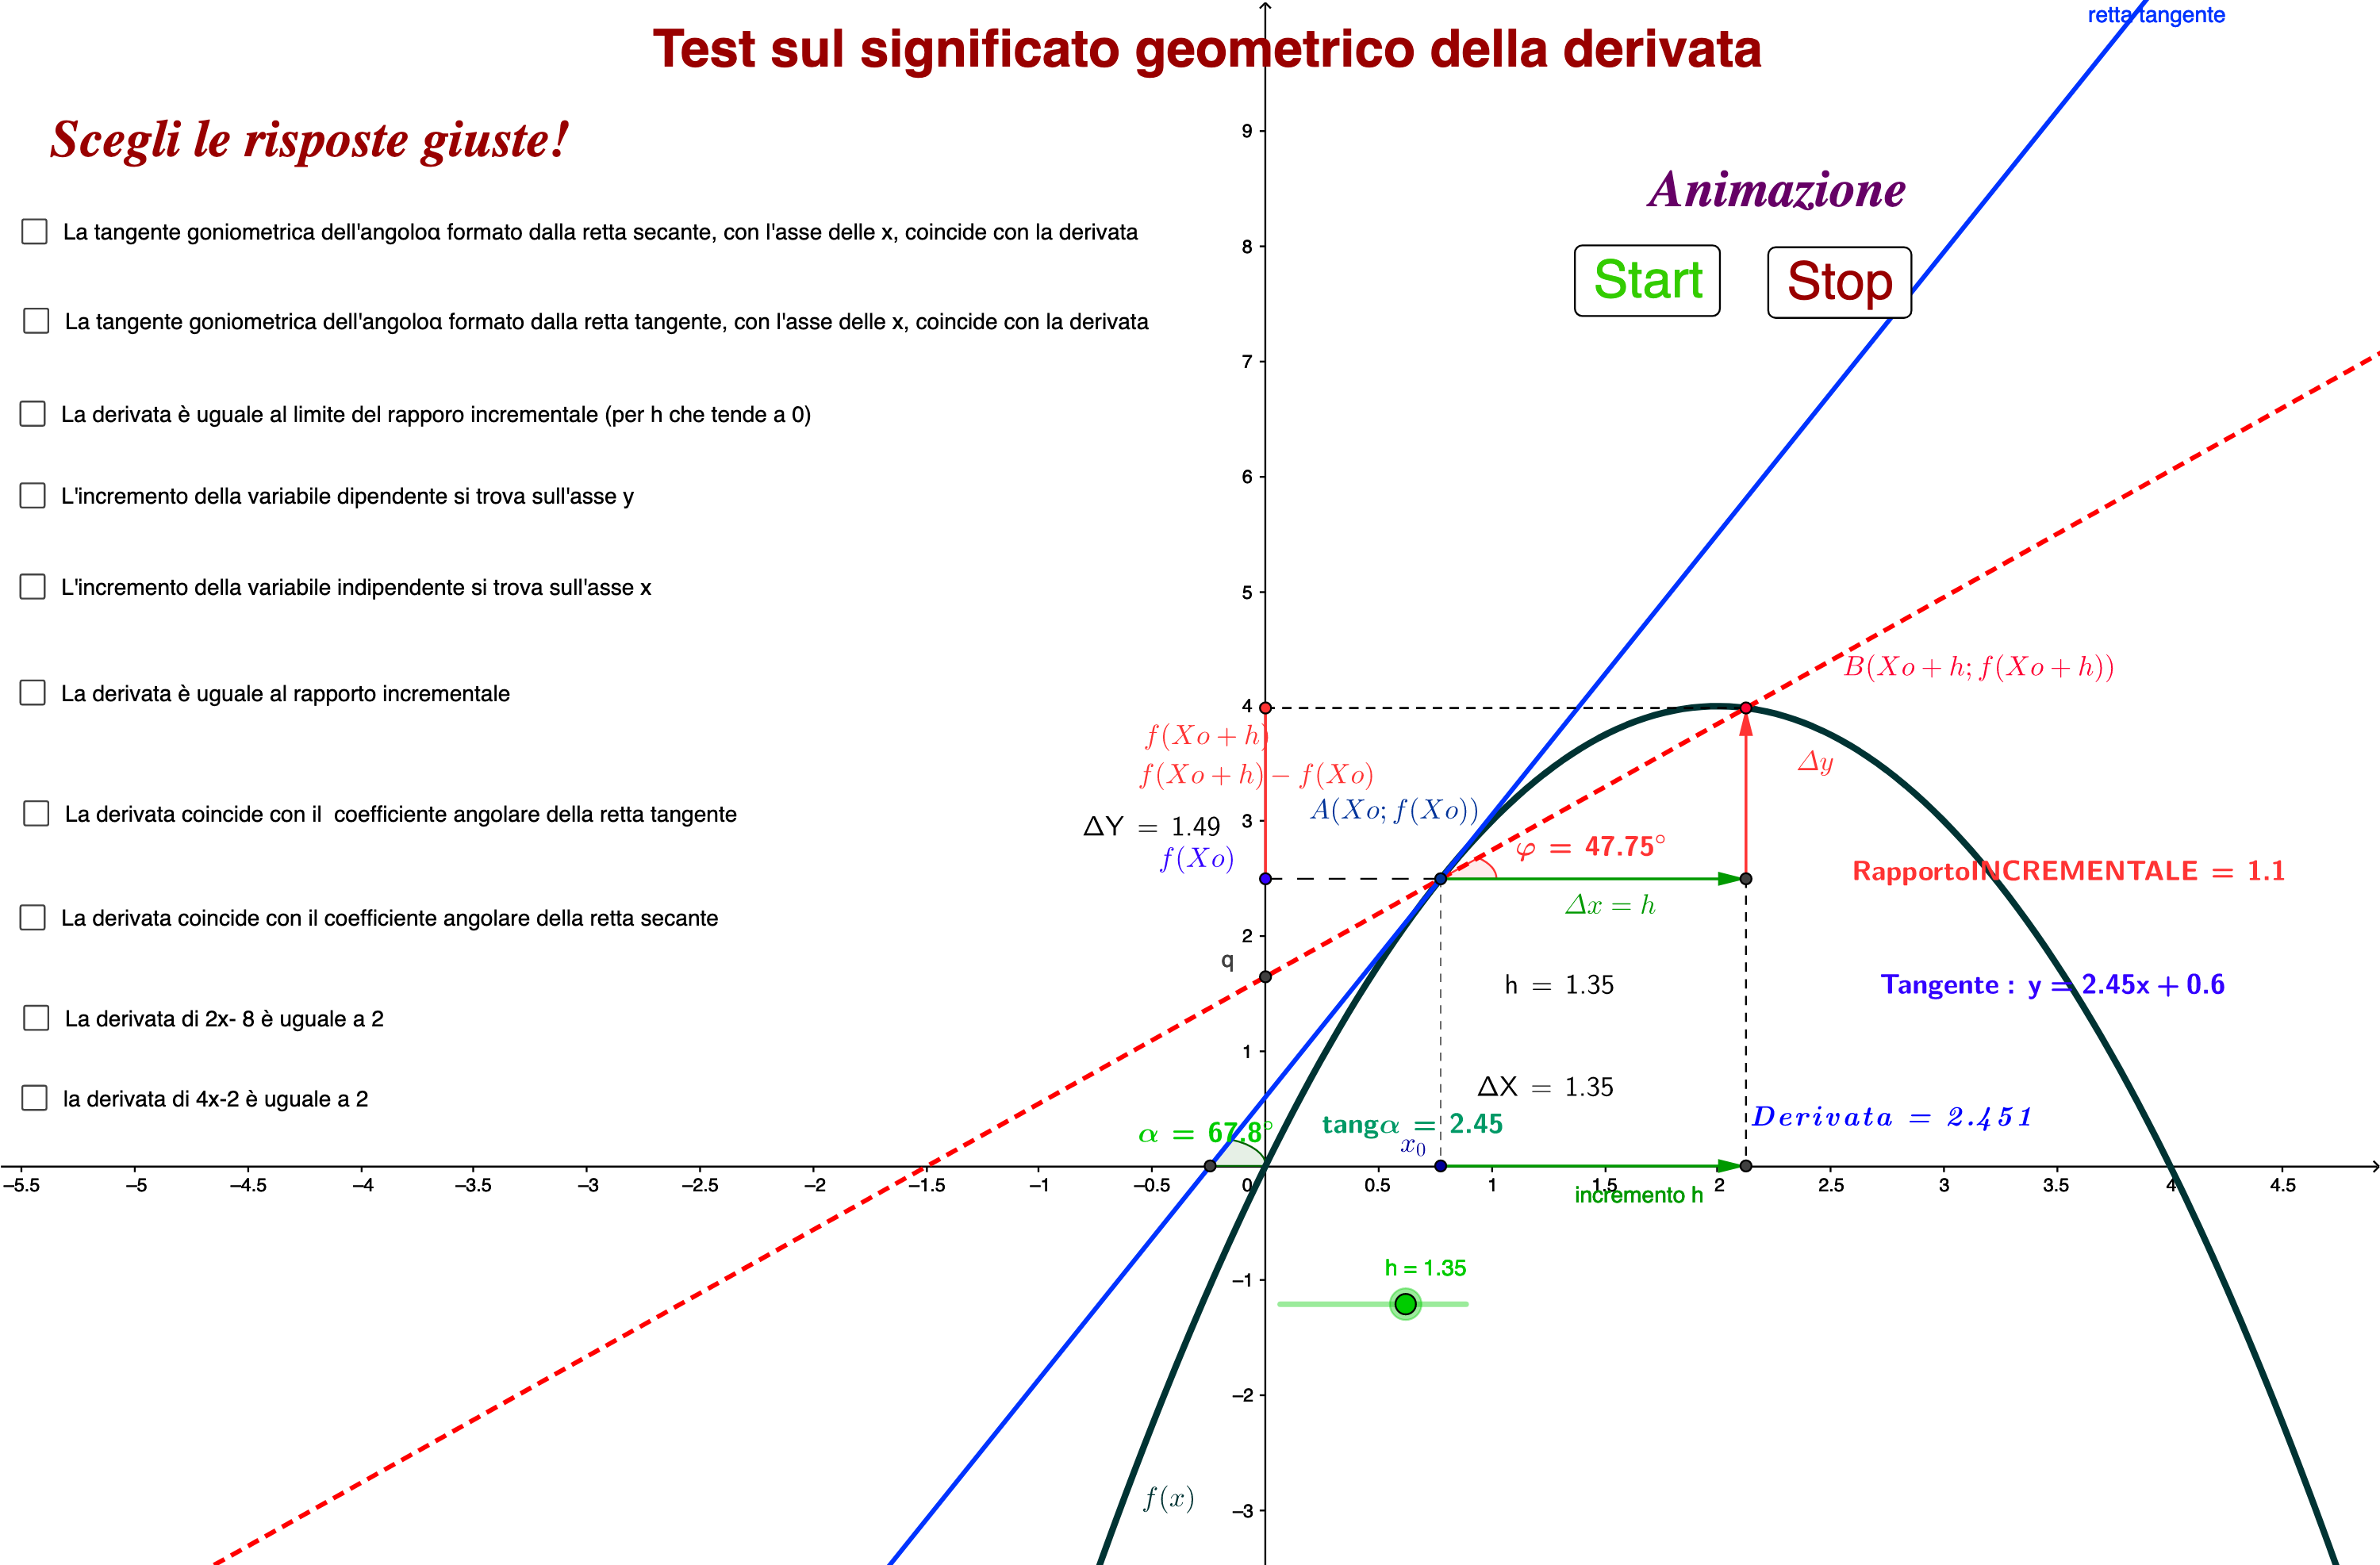
\includegraphics[scale=0.6]{derivata}\\ 
\end{multicols}
\end{frame}

\begin{frame}[t]{Esercizi sulle derivate} \vspace{10pt}
\begin{theorem}[Pythagoras] \vspace{2pt}
$ a^2 + b^2 = c^2$
\end{theorem}
\begin{corollary} \vspace{2pt}
$ x + y = y + x  $
\end{corollary}

\begin{proof} \vspace{2pt}
$\omega +\phi = \epsilon $
\end{proof}
\end{frame}

\begin{frame}[t]{Rappresentazione Grafica delle Derivata} \vspace{10pt}
\begin{center}
	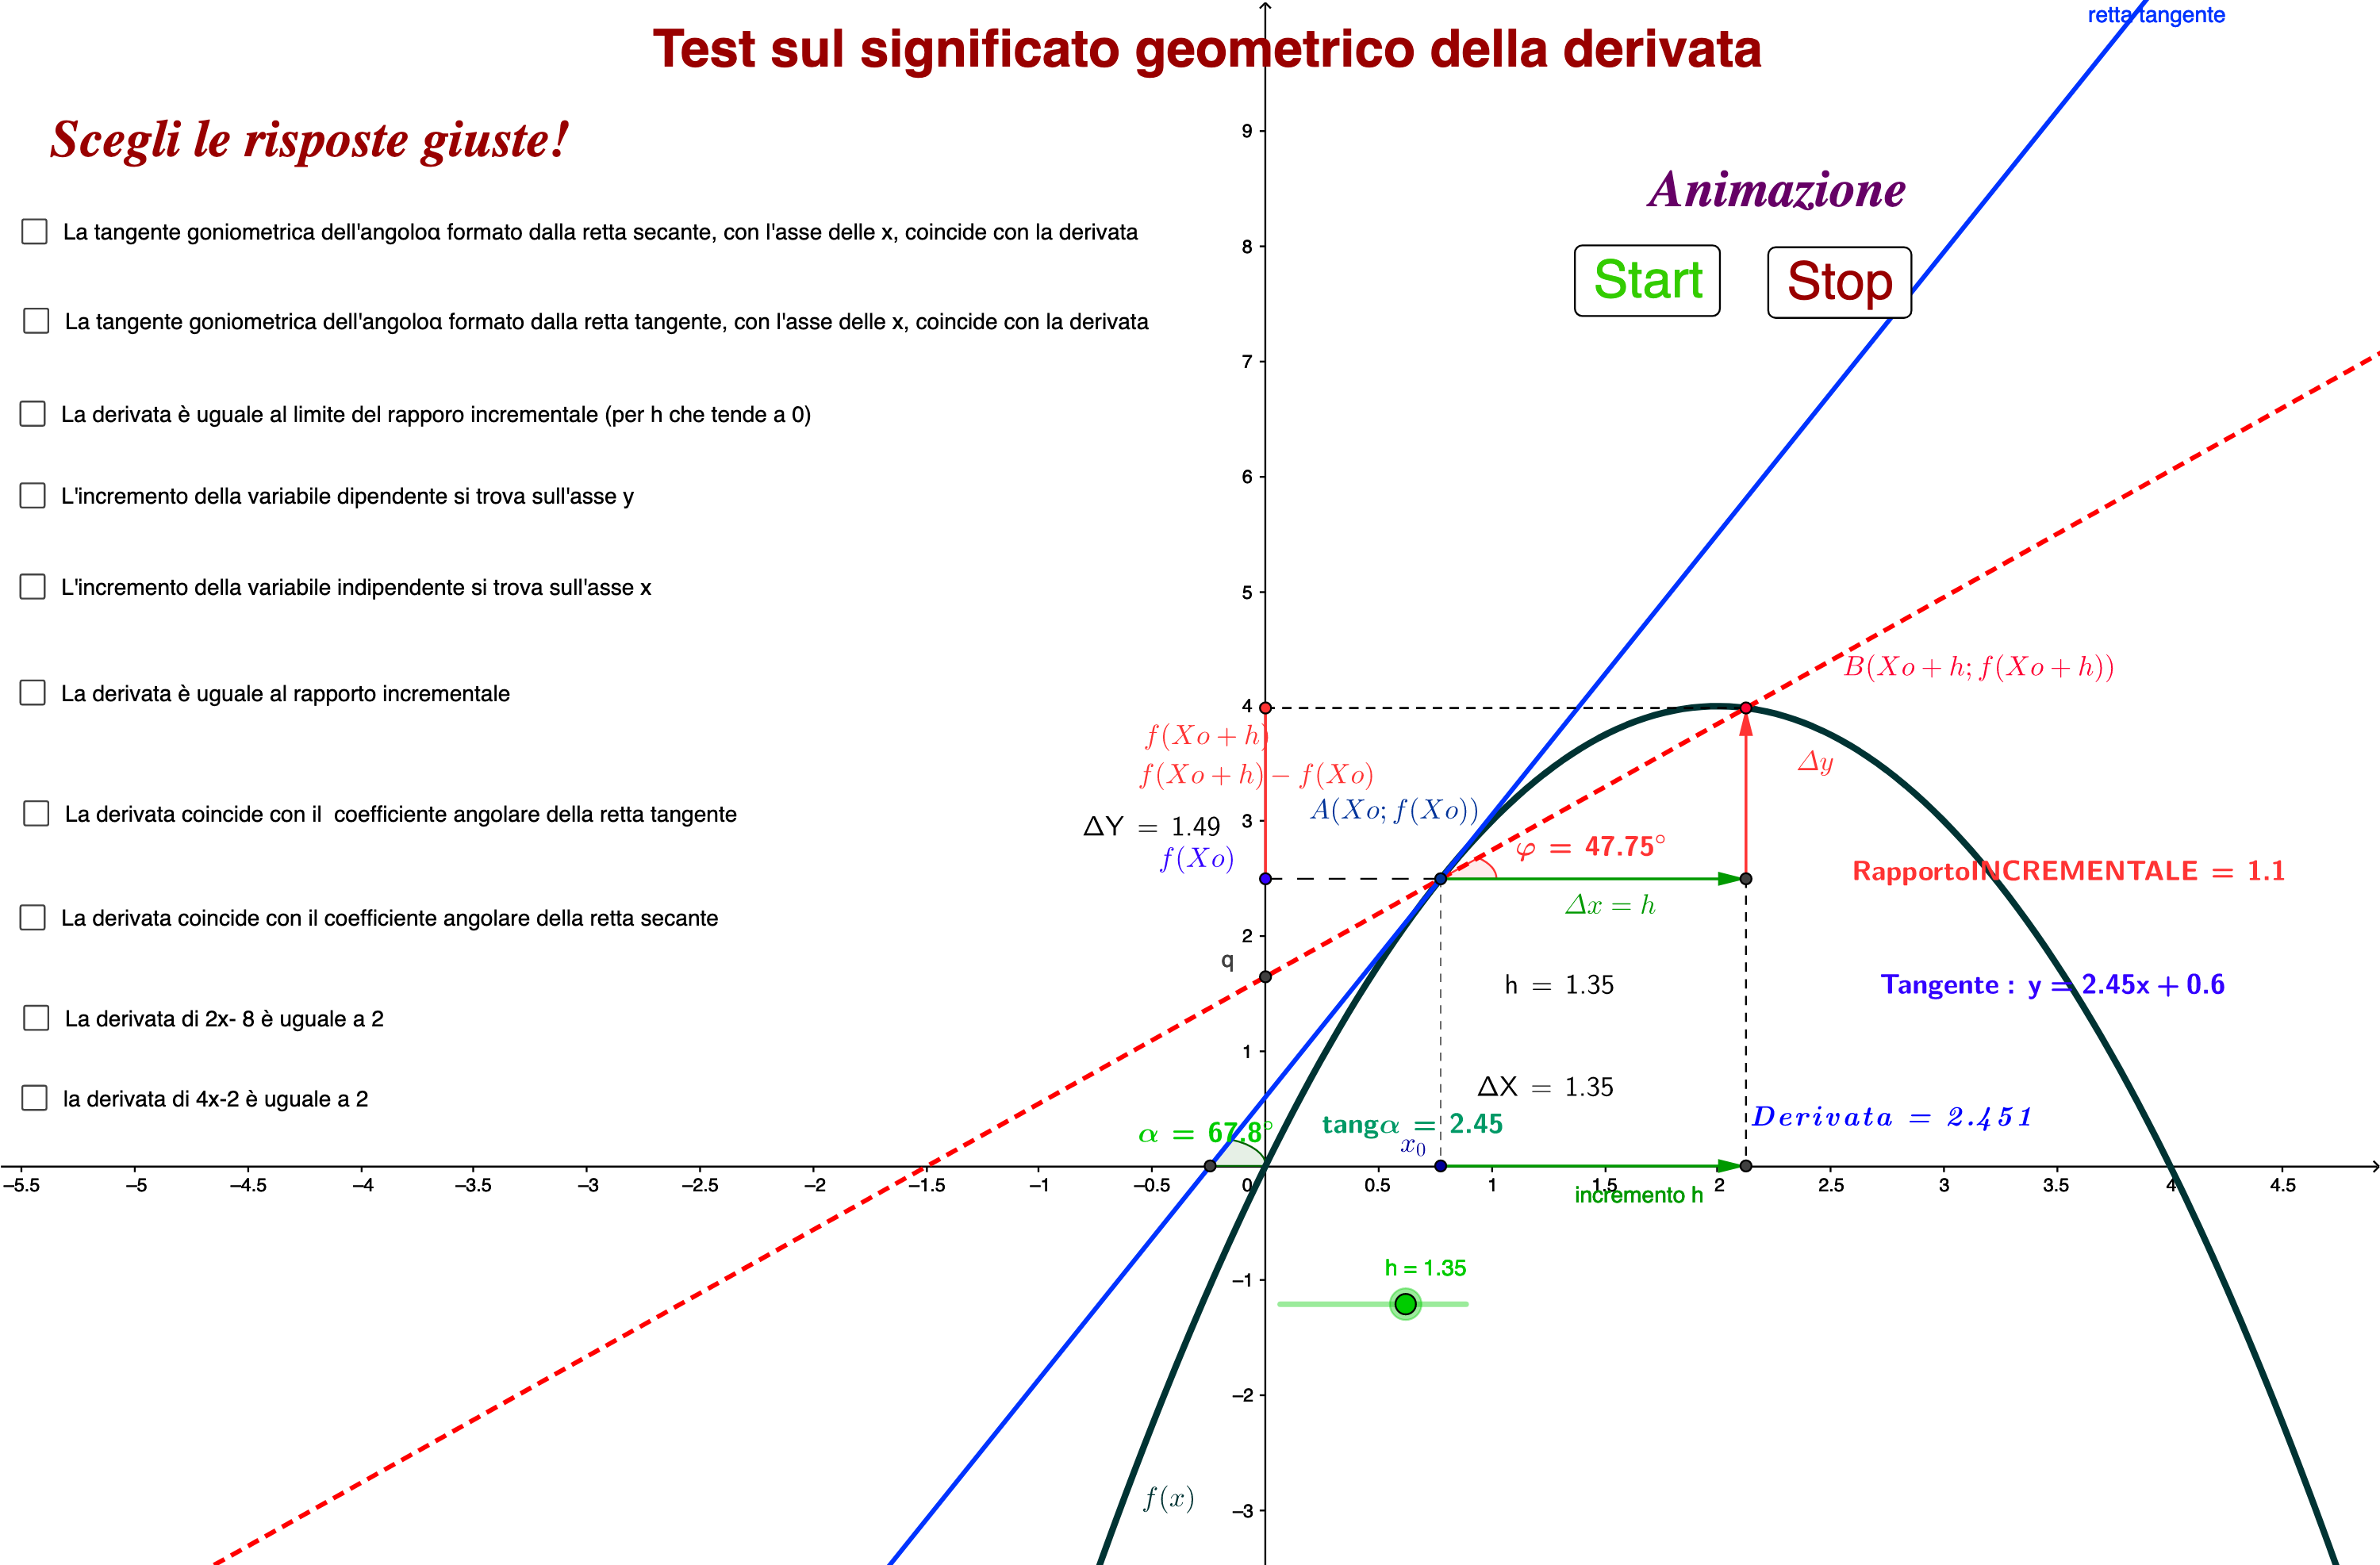
\includegraphics[scale=0.90]{derivata}
\end{center}
\end{frame}
\section{Compiti per casa}

\begin{frame}[t]{Esercizi sulle derivate} 
\vspace{10pt}

\begin{alertblock}{cosa studiare} \vspace{2pt}
Lorem ipsum dolor sit amet, consectetur adipisicing elit, 
sed do eiusmod tempor incididunt ut labore et 
dolore magna aliqua.
\end{alertblock}

\pause

\begin{alertblock}{come studiare} \vspace{2pt}
Lorem ipsum dolor sit amet, consectetur adipisicing elit, 
sed do eiusmod tempor incididunt ut labore et 
dolore magna aliqua.
\end{alertblock}

\pause

\begin{alertblock}{esrcizi - revisione} \vspace{2pt}
Lorem ipsum dolor sit amet, consectetur adipisicing elit, 
sed do eiusmod tempor incididunt ut labore et 
dolore magna aliqua.
\end{alertblock}

\end{frame}

\begin{frame}[t]{Rappresentazione Grafica delle Derivata}
\vspace{2cm}
\begin{center}
	\huge {\bf \textcolor{cyan}{buon lavoro!}}
\end{center}
\end{frame}

\end{document}